\chapter{Räumliches Lernen auf Graphen}
\label{raeumliches_lernen}

Spatially sliding a filter on the vertices, as you would slide a filter on a 2D image or a 1D audio signal (the pixels form a grid graph, the time forms a line graph), i.e. the straightforward application of the definition of a convolution. This approach however presents two challenges: (1) the definition of a receptive field / neighbourhood, because sampling on arbitrary graphs is not necessarily uniform and (2), the ordering of nodes, because problem-specific ordering, e.g. spatially ordered pixels or time ordered samples, is missing. These recent works, who present the same ideas differently, spatially define the convolution operator on graphs:


\section{Spektrale Graphentheorie}
\label{spektrale_graphentheorie}

Es gibt 2 große Quellen hier:
\begin{itemize}
  \item Spectral Graph Theory by Chung
  \item Discrete Laplace-Beltrami Operator
\end{itemize}
+ 5 zum Lernen:
\begin{itemize}
  \item Semi Supervised Classification
  \item Fast Localized Spectral Filterung
  \item Wavelets on Graphs via Spectral Graph Theory
  \item The Emerging Field of Signal Processing on Graphs
  \item How powerful are Graph Convolutions? (Review)
\end{itemize}

\subsection{Eigenwerte und Eigenvektoren reell symmetrischer Matrizen}
\label{eigenwerte_symmetrischer_matrizen}

\todo{intro}

$\ma{M} \in \gls{R}^{N \times N}$.
$\gls{eiv} \in \gls{R}^{N}$, $\gls{eiv} \neq \mathbf{0}$.
$\gls{lambda} \in \gls{R}$.
\emph{Eigenwertproblem} $\ma{M}\gls{eiv} = \gls{lambda}\gls{eiv}$.
Zu einem \emph{Eigenwert} $\gls{lambda}$ gibt es unendlich viele (skalierte) \emph{Eigenvektoren} \gls{eiv}.
Wir definieren den Eigenvektor \gls{eiv} eines Eigenwertes \gls{lambda} daher eindeutig über die Bedingung $\left\|\gls{eiv}\right\|_2 = 1$.
Sei \ma{M} weiterhin symmetrisch, \dhe{} $\ma{M} = \ma{M}^{\top}$.
Dann gilt für zwei unterschiedliche Eigenvektoren $\gls{eiv}_1$ und $\gls{eiv}_2$, dass $\gls{eiv}_1 \gls{ortho} \gls{eiv}_2$.
Weiterhin hat \ma{M} genau $N$ reelle Eigenwerte mit ${\left\{\gls{lambda}_i\right\}}_{i=1}^N$.

Wir definieren zu \ma{M} die orthogonale \emph{Eigenvektormatrix} $\gls{Eiv} = \left[\gls{eiv}_1, \ldots, \gls{eiv}_n\right] \in \gls{R}^{N \times N}$, wobei $\gls{Eiv}\gls{Eiv}^{\top}=\gls{I}$, und dessen korrespondierende Eigenwertdiagonalmatrix $\gls{Lambda} = \gls{diag}\left(\left[\gls{lambda}_1, \ldots, \gls{lambda}_N\right]\right)$, \dhe{} $\gls{Lambda}_{ii} = \gls{lambda}_i$.
Dann gilt $\ma{M}\gls{Eiv} = \gls{Eiv}\gls{Lambda}$ und insbesondere ist \ma{M} diagonalisierbar über
\begin{equation}
  \ma{M} = \ma{M}\gls{Eiv}\gls{Eiv}^{\top} = \gls{Eiv}\gls{Lambda}\gls{Eiv}^{\top}.
\end{equation}

Weiterhin gilt für die $k$te Potenz von $\ma{M}$, $k \in \gls{N}$,
\begin{equation}
  \ma{M}^k = {\left(\gls{Eiv}\gls{Lambda}\gls{Eiv}^{\top}\right)}^k = \gls{Eiv}\gls{Lambda}^k\gls{Eiv}^{\top}.
\end{equation}

Dieser Zusammenhang lässt sich verdeutlichen, wenn man die Potenz ausschreibt:
\begin{equation*}
  {\left(\gls{Eiv}\gls{Lambda}\gls{Eiv}^{\top}\right)}^k = \gls{Eiv}\gls{Lambda}\gls{Eiv}^{\top}\gls{Eiv}\gls{Lambda}\gls{Eiv}^{\top}\prod^{k-2}_{i=1} \gls{Eiv}\gls{Lambda}\gls{Eiv}^{\top} = \gls{Eiv}\gls{Lambda}^2\gls{Eiv}^{\top} \prod^{k-2}_{i=1} \gls{Eiv}\gls{Lambda}\gls{Eiv}^{\top} = \gls{Eiv}\gls{Lambda}^k \gls{Eiv}^{\top}.
\end{equation*}

Falls \ma{M} weiterhin \emph{schwach diagonaldominant} ist, \dhe{}
\begin{equation}
  \sum_{\substack{j=1\\j \neq i}}^N \left|\ma{M}_{ij}\right| \leq \left|\ma{M}\right|_{ii},
  \label{eq:schwach_diagonaldominant}
\end{equation}
und $\ma{M}_{ii} \geq 0$ für alle $i \in \left\{1, \ldots, N\right\}$, ist \ma{M} \emph{positiv semidefinit}, \dhe{} $\ve{x}^{\top}\ma{M}\ve{x} \geq 0$ für alle $\ve{x} \in \gls{R}^{N}$.
Eigenwerte symmetrischer positiv semidefiniter Matrizen $\lambda_i \in \gls{R+}$ sind positiv reell und es lässt sich folglich auf diesen eine Ordnung definieren mit $0 \leq \gls{lambda}_1 \leq \cdots \leq \gls{lambda}_N \coloneqq \gls{lambdamax}$.

\todo{quelle}

\subsection{Laplace-Matrix}
\label{laplace_matrix}

Our eigenvalues relate well to other graph invariants for general graphs in a way that other definitions (such as the eigenvalues of adjacency matrices) often fail to do.
The advantages of this definition are perhaps due to the fact that it is consistent with the eigenvalues in spectral geometry and in stochastic processes.
Many results which were only known for regular graphs can be generalized to all graphs~\cite{Chung}.

\todo{intro}

Für einen schleifenlosen, ungerichteteten, gewichtet oder ungewichteten Graphen \gls{G} und dessen Adjazenzmatrix \gls{A} mit Gradmatrix \gls{D} ist die \emph{kombinatorische Laplace-Matrix} \gls{L} definiert als $\gls{L} = \gls{D} - \gls{A}$~\cite{Chung}.
Die \emph{normalisierte Laplace-Matrix} \gls{Lnorm} ist definiert als $\gls{Lnorm} = \gls{D}^{-\frac{1}{2}} \gls{L} \gls{D}^{-\frac{1}{2}}$ mit der Konvention, dass $\gls{D}^{-\frac{1}{2}}_{ii} = 0$ für isolierte Knoten $\gls{v}_i \in \gls{V}$ in \gls{G}, \dhe{} $\gls{D}_{ii} = 0$~\cite{Chung}.
Daraus ergibt sich die elementweise Definition
\begin{equation*}
  \gls{Lnorm}_{ij} = \begin{cases}
  1, & \text{wenn }i = j,\\
    -\frac{\gls{w}\left(\gls{v}_i, \gls{v}_j\right)}{\sqrt{\gls{d}\left(\gls{v}_i\right)\gls{d}\left(\gls{v}_j\right)}}, & \text{wenn }\gls{v}_i \gls{adj} \gls{v}_j,\\
  0, & \text{sonst.}
\end{cases}
\end{equation*}
Für verbundene Graphen kann \gls{Lnorm} vereinfacht werden zu $\gls{Lnorm} = \gls{I} - \gls{D}^{-\frac{1}{2}} \gls{A} \gls{D}^{-\frac{1}{2}}$~\cite{Chung}.
Jeder Eintrag auf der Diagonalen der normalisierten Laplace-Matrix ist folglich Eins.
\gls{Lnorm} ist damit normalisiert auf den (gewichteten) Grad zweier adjazenter Knoten $\gls{v}_i$ und $\gls{v}_j$.
Es ist anzumerken, dass \gls{L} und insbesondere \gls{Lnorm} symmetrisch sind, wohingegen eine Normalisierung der Form $\gls{D}^{-1}\gls{L}$ dies in der Regel nicht wäre~\cite{Reuter}.

\gls{L} und \gls{Lnorm} sind keine ähnlichen Matrizen.
Insbesondere sind ihre Eigenvektoren unterschiedlich.
Die Nutzung von \gls{L} oder \gls{Lnorm} ist damit abhängig von dem Problem, welches man betrachtet~\cite{Hammond}.
Wir schreiben \gls{Lboth} wenn die Wahl der Laplace-Matrix, ob \gls{L} oder \gls{Lnorm}, für die weitere Berechnung zwar fest, aber irrelevant ist.

\paragraph{Interpretation}
\label{laplace_interpretation}

\todo{kurz laplace beltrami}

Sei $\ve{f} \in \gls{R}^N$ eine Funktion \bzw{} ein Signal auf den Knoten eines Graphen \gls{G}.
Dann kann für die kombinatorische Laplace-Matrix \gls{L} verifiziert werden, dass \gls{L} die Gleichung
\begin{equation*}
  {\left(\gls{L}\ve{f}\right)}_i = \sum_{i \gls{adj} j} \gls{w}\left(\gls{v}_i, \gls{v}_j\right) \left(\ve{f}_i - \ve{f}_j\right)
\end{equation*}
erfüllt~\cite{Hammond}.
Sei $\gls{G}$ nun ein Graph, der aus einem (unendlichen) zweidimensionalen regulärem Gitter entstanden ist, \dhe{} jeder Knoten $\gls{v}_i$ besitzt genau $4$ Nachbarn mit gleichen Kantengewichten $\frac{1}{\delta^2}$, wobei $\delta \in \gls{R}$ beliebige Konstante.
Zur einfacheren Veranschaulichung benutzen wir dabei für die Signalstärke $\ve{f}_i$ eines Knoten $v_i$ an Position $\left(x, y\right)$ die Indexnotation $\ve{f}_{x,y}$.
Dann beschreibt
\begin{equation*}
  {\left(\gls{L}\ve{f}\right)}_{x,y} = \frac{4\ve{f}_{x,y} - \ve{f}_{x+1,y} - \ve{f}_{x-1,y} - \ve{f}_{x,y+1} - \ve{f}_{x,y-1}}{h^2}
\end{equation*}
die \emph{5-Punkte-Stern} Approximation $-\nabla^2 f$ (bei umgekehrtem Vorzeichen) definiert auf den Punkten $\left\{\left(x,y\right), \left(x+\delta,y\right), \left(x-\delta,y\right), \left(x,\delta+h\right),\left(x,y-\delta\right)\right\}$~\cite{Hammond}.\todo{grafik}
Ähnlich zu einem regulären Gitter lässt sich ein Graph \gls{G} auch über beliebig viele Abtastpunkte einer differenzierbaren Mannigfaltigkeit konstruieren.
Es zeigt sich, dass mit steigender Abtastdichte und geeigneter Wahl der Kantengewichte die normalisierte Laplace-Matrix \gls{Lnorm} zu dem kontinuierlichem Laplace-Beltrami Operator konvergiert~\cite{Hammond}.
Damit kann $\gls{Lnorm}$ als die diskrete Analogie des $\nabla^2$ Operators auf Graphen verstanden werden.
Der Laplace-Beltrami Operator misst dabei, in wie weit sich eine Funktion $f$ an einem Punkt $x$ von dem Durchschnitt aller Funktionspunkte um einen kleinen Bereich um $x$ unterscheidet.
Die Laplace-Matrix operiert dabei völlig analog, in dem sie misst, wie sehr sich eine (diskrete) Funktion um einen Knoten im Vergleich zu seinen Nachbarknoten unterscheidet.

Eigenwerte und Eigenvektoren von \gls{Lboth} helfen uns dabei, die lineare Transformation einer Funktion \ve{f} (mehrfach) angewendet auf \gls{Lboth} besser zu verstehen.
Wir können dafür \ve{f} als Linearkombination der Eigenbasis $\sum_i c_i \gls{eiv}_i$ schreiben und erhalten
\begin{equation*}
  \gls{Lboth}^k \ve{f} = \sum_i c_i \gls{Lboth}^k \gls{eiv}_i = \sum_i c_i \gls{lambda}_i^k \gls{eiv}_i.
\end{equation*}
Somit können Eigenschaften von \gls{Lboth} und damit des Graphen selber durch dessen Eigenwerte und Eigenvektoren beschrieben werden.

\paragraph{Eigenschaften}
\label{laplace_eigenschaften}

$\gls{Lboth} \in \gls{R}^{N \times N}$ ist eine reell symmetrisch, positiv semidefinite Matrix~\cite{Chung}.
Folglich besitzt \gls{Lboth} nach Kapitel~\ref{eigenwerte_symmetrischer_matrizen} genau $N$ positiv reelle Eigenwerte ${\left\{\gls{lambda}_i\right\}}_{i=1}^N$ mit Ordnung $0 \leq \gls{lambda}_1 \leq \cdots \leq \gls{lambda}_N$ und $N$ korrespondierende orthogonale Eigenvektoren ${\left\{\gls{eiv}_i\right\}}_{i=1}^N$.

Die kombinatorische Laplace-Matrix $\gls{L}$ ist nach~\eqref{eq:schwach_diagonaldominant} weiterhin schwach diagonaldominant.
Insbesondere summiert sich jede Reihen- und Spaltensumme von \gls{L} zu Null auf, \dhe{} $\sum_{j=1}^N \gls{L}_{ij} = \sum_{j=1}^N \gls{L}_{ji} = 0$.
Daraus folgt unmittelbar, dass $\gls{lambda}_1 = 0$, da $\gls{eiv}_1 = \frac{1}{\sqrt{N}}{\left[1, \ldots, 1\right]}^{\top} \in \gls{R}^N$ Eigenvektor von \gls{L} mit $\gls{L}\gls{eiv}_1 = \ve{0}$.
\gls{Lnorm} hingegen ist nicht zwingend schwach diagonaldominant.
Es lässt sich jedoch zeigen, dass auch für \gls{Lnorm} gilt, dass $\gls{lambda}_1 = 0$~\cite{Chung}.

Eine der interessantesten Eigenschaften eines Graphs ist dessen Konnektivität.
Die Laplace-Matrix \gls{Lboth} \bzw{} dessen Eigenwerte stellen ein geeignetes Mittel zur Untersuchung dieser Eigenschaft dar.
So gilt \zB{} für einen verbundenen Graphen \gls{G}, dass $\gls{lambda}_2 > 0$.
Falls $\gls{lambda}_i = 0$ und $\gls{lambda}_{i+1} \neq 0$, dann besitzt $\gls{G}$ genau $i$ verbundene Komponenten~\cite{Chung}.
Damit ist die Anzahl der Null-Eigenwerte äquivalent zu der Anzahl an Komponenten, die ein Graph besitzt.
Für \gls{Lnorm} lässt sich weiterhin zeigen, dass $\gls{lambdamax} \leq 2$ eine obere Schranke ihrer Eigenwerte ist~\cite{Chung}.

Aus der Laplace-Matrix können ebenso Rückschlüsse über die kürzeste Pfadlänge zweier Knoten gewonnen werden.
So gilt für $\gls{Lboth}^{k}$ mit $k \in \gls{N}$, dass $\gls{Lboth}^k_{ij} = 0$ genau dann, wenn $\gls{s}\left(v_i, v_j\right) > k$~\cite{Hammond}.
Damit beschreibt $\gls{Lboth}^k_i$ bildlich gesprochen die Menge an Knoten, die maximal $k$ Kanten von $i$ entfernt liegen.

\section{Spektraler Faltungsoperator}
\label{spektraler_faltungsoperator}

Sei $\ve{f} \in \gls{R}^N$ ein Signal auf den Knoten eines Graphen \gls{G}, welches abhängig von der Struktur des Graphen weiter verarbeitet werden soll.
Es ist jedoch nicht selbstverständlich, wie recht einfache, dennoch fundamentale Signalverarbeitungsprozesse wie Translation oder Filterung und die daraus entstehende Faltung in der Domäne des Graphen definiert werden können~\cite{Shuman}.
So kann \zB{} ein analoges Signal $f\left(t\right)$ mittels $f\left(t-3\right)$ um $3$ nach rechts verschoben werden.
Es ist hingegen völlig unklar was es bedeutet, ein Graphsignal auf den Knoten um $3$ nach rechts zu bewegen (\vgl{}~\cite{Shuman}).
Die spektrale Graphentheorie bietet uns dafür einen geeigneten Weg, in dem Eingabesignale in das Spektrum des Graphen zerlegt \bzw{} abgebildet, modifiziert und wieder retransformiert werden können.

\subsection{Graph-Fourier-Transformation}
\label{graph_fourier_transformation}

Das Spektrum eines Graphen \gls{G} bilden die Eigenwerte ${\left\{\gls{lambda}_i\right\}}_{i=1}^N$ der Laplace-Matrix \gls{Lboth} von \gls{G}.
Diese werden deshalb auch oft als die \emph{Frequenzen} von \gls{G} betitelt.
In der spektralen Domäne können wir ein Eingabeignal \ve{f} über \gls{G} dann analog wie ein zeitdiskretes Abtastsignal in der Fourier-Domäne behandeln.

\paragraph{Klassische Fourier-Transformation}
\label{klassische_fourier_transformation}

Die Fourier-Transformation $\hat f$ einer Funktion $f\left(t\right)$ ist definiert als~\cite{Shuman}
\begin{equation*}
  \hat f\left(\omega\right) \coloneqq \left\langle f, e^{2\pi i\omega t} \right\rangle = \int_{\gls{R}} f\left(t\right)e^{-2\pi i\omega t}\,\mathrm{d}t.
\end{equation*}
Die komplexen Exponentiale $e^{2\pi i\omega t}$ beschreiben dabei die Eigenfunktionen des eindimensionalen Laplace-Beltrami Operators~\cite{Shuman}
\begin{equation}
  - \nabla^2 e^{2\pi i\omega t} = - \frac{\partial^2}{\partial t^2} e^{2\pi i \omega t} = {\left(2\pi \omega\right)}^2 e^{2\pi i\omega t}.
  \label{eq:laplace_eigenfunktionen}
\end{equation}
$\hat f$ kann damit als die Ausdehnung von $f$ in Bezug auf die Eigenfunktionen des Laplace-Beltrami Operators $\nabla^2$ verstanden werden~\cite{Hammond}.
\\\\
Analog lässt sich die \emph{Graph-Fourier-Transformation} einer Funktion $f \colon \gls{V} \to \gls{R}$ \bzw{} $\ve{f} \in \gls{R}^N$ auf den Knoten eines Graphen \gls{G} als Ausdehnung von $f$ in Bezug auf die Eigenvektoren ${\left\{\gls{eiv}_i\right\}}_{i=1}^N$ der Laplace-Matrix \gls{Lboth} definieren~\cite{Shuman}:
\begin{equation}
  \hat f\left(\gls{lambda}_i\right) \coloneqq \left\langle \ve{f}, \gls{eiv}_i \right\rangle\, \text{\bzw{} } \ve{\hat f} \coloneqq \gls{Eiv}^{\top}\ve{f}.
  \label{eq:graph_fourier_transformation}
\end{equation}
Die inverse Graph-Fourier-Transformation ergibt sich dann als~\cite{Shuman}
\begin{equation}
  f\left(\gls{v}_i\right) = \sum_{j=1}^N \hat f\left(\gls{lambda}_j\right) {\left(\gls{eiv}_j\right)}_i\,\text{\bzw{} }\ve{f} = \gls{Eiv}\ve{\hat f}.
  \label{eq:inverse_graph_fourier_transformation}
\end{equation}

In der klassischen Fourier-Analyse sind für die Eigenwerte ${\left\{{\left(2\pi \omega\right)}^2\right\}}_{\omega \in \gls{R}}$ in~\eqref{eq:laplace_eigenfunktionen} nahe bei Null die korrespondieren Eigenfunktionen kleine, weich schwingende Funktionen, wohingegen für größere Eigenwerte \bzw{} Frequenzen die Eigenfunktionen sehr schnell und zügig anfangen zu oszillieren.
Bei der Graph-Fourier-Transformation ist dies ähnlich.
So ist für \gls{L} der erste Eigenvektor $\gls{eiv}_1 = \frac{1}{\sqrt{N}}{\left[1, \ldots, 1\right]}^{\top}$ zum Eigenwert $\gls{lambda}_1 = 0$ konstant und an jedem Knoten gleich.
Generell zeigt sich, dass die Eigenvektoren geringer Frequenzen nur geringfügig im Graph variieren, wohingegen Eigenvektoren größerer Eigenwerte immer unähnlicher werden (\vgl{}~\cite{Shuman}).
\\\\
Die Graph-Fourier-Transformation~\eqref{eq:graph_fourier_transformation} und ihre Inverse~\eqref{eq:inverse_graph_fourier_transformation} bieten uns eine Möglichkeit ein Signal in zwei unterschiedlichen Domänen zu repräsentieren, nämlich der Knotendomäne, \dhe{} das unveränderte Signal auf der Knotenmenge $f\left(\gls{v}_i\right)$, und der spektralen Domäne, \dhe{} das transformierte Signal in das Spektrum des Graphen $\hat f\left(\gls{lambda}_i\right)$.
Diese Transformation erlaubt uns die Formulierung fundamentaler Signalverarbeitungsoperationen.

\subsection{Spektrale Filterung}
\label{spektrale_filterung}

In der Signalverarbeitung versteht man unter der Frequenzfilterung die Transformation eines Eingabesignals in die Fourier-Domäne und der verstärkenden oder dämpfenden Veränderung der Amplituden der Frequenzkomponenten.
Formal betrachtet ergibt dies
\begin{equation}
  \hat f_{\mathrm{out}}\left(\omega\right) \coloneqq \hat f_{\mathrm{in}}\left(\omega\right)\hat g\left(\omega\right)
  \label{eq:fourier_filtering}
\end{equation}
mit dem Filter $\hat g \colon \gls{R} \to \gls{R}$.
\citeauthor{Shuman} zeigen, dass die Filterung in der Fourier-Domäne äquivalent zu einer Faltung in der Zeitdomäne ist, \dhe{}
\begin{equation}
  \left(f_{\mathrm{in}} \star g\right)\left(t\right) \coloneqq \int_{\gls{R}} f_{\mathrm{in}}\left(\tau\right)g\left(t - \tau\right)\, \mathrm{d}\tau = f_{\mathrm{out}}\left(t\right).
  \label{eq:fourier_faltung}
\end{equation}

Wir können die Filterung der Frequenzen in der Fourier-Domäne analog zu~\eqref{eq:fourier_filtering} für die spektrale Domäne auf Graphen über
\begin{equation*}
  \hat f_{\mathrm{out}}\left(\gls{lambda}_i\right) \coloneqq \hat f_{\mathrm{in}}\left(\gls{lambda}_i\right)\hat g\left(\lambda_i\right)\,\text{\bzw{} }\ve{\hat f}_{\mathrm{out}} \coloneqq \ve{\hat f}_{\mathrm{in}} \gls{hadamard} \ve{\hat g}
\end{equation*}
beschreiben, wobei \gls{hadamard} das elementweise Hadamard-Produkt ist~\cite{Shuman}.
$\ve{\hat g} \in \gls{R}^N$ ist damit ein \emph{nicht-parametrischer} Filter, \dhe{} ein Filter, dessen Werte für alle Frequenzen ${\left\{\gls{lambda}_i\right\}}_{i=1}^N$ frei wählbar sind~\cite{Defferrard}.
Daraus ergibt sich analog zu~\eqref{eq:fourier_faltung} der \emph{spektrale Faltungsoperator} auf Graphen in der Knotendomäne mit Hilfe der Graph-Fourier-Transformation~\eqref{eq:graph_fourier_transformation} und ihrer Inversen~\eqref{eq:inverse_graph_fourier_transformation} als~\cite{Shuman, Defferrard}
\begin{equation}
  \ve{f}_{\mathrm{in}} \star \ve{\hat g} \coloneqq \gls{Eiv}\left(\gls{Eiv}^{\top}\ve{f}_{\mathrm{in}} \gls{hadamard} \ve{\hat g}\right) = \ve{f}_{\mathrm{out}}.
  \label{eq:spektraler_faltungsoperator}
\end{equation}

\subsection{Polynomielle Approximation}
\label{polynomielle_approximation}

Es zeigt sich, dass die Benutzung des spektralen Faltungsoperators in~\eqref{eq:spektraler_faltungsoperator} im Kontext eines \glspl{CNN} auf Graphen mehrere Schwächen aufweist.
Es ist \zB{} leicht ersichtlich, dass die Auswertung von $\ve{f}_{\mathrm{in}} \star \ve{\hat g}$ extrem berechnungsintensiv ist.
So liegt die Laufzeit der Multiplikation mit der dichtbesetzten Eigenvektormatrix \gls{Eiv} in $\gls{O}\left(N^2\right)$, zudem muss \gls{Eiv} zuerst bestimmt werden — ein kostspieliger Aufwand für Graphen mit möglicherweise weit mehr als hundert Knoten~\cite{gcn}.
Desweiteren führt ein Filter $\ve{\hat g} \in \gls{R}^N$ der Größe $N$ zu einem Lernaufwand in $\gls{O}\left(N\right)$, \dhe{} der Dimensionalität der Eingabedaten~\cite{Defferrard}.
Ebenso kann $\ve{\hat g}$ so nicht für das Lernen auf unterschiedlich großen Graphen verwendet werden.

Um die oben genannten Schwächen zu umgehen kann $\hat g\left(\gls{lambda}_i\right)$ über ein Polynom\begin{equation}
  \hat g\left(\gls{lambda}_i\right) \approx \sum_{k=0}^K c_k\gls{lambda}_i^k \eqqcolon \hat g^{\prime}\left(\gls{lambda}\right)
  \label{eq:spektraler_filter_approximation}
\end{equation}
vom Grad $K$ mit Koeffizienten $c_0, \ldots, c_K \in \gls{R}$ approximiert werden~\cite{Hammond, Defferrard}.
Die Filtergröße von $\hat g^{\prime}$ sinkt somit auf einen konstanten Faktor $K$ mit Lernaufwand $\gls{O}\left(K\right)$, \dhe{} dem gleichen Aufwand klassischer zweidimensionaler \glspl{CNN}~\cite{Defferrard}.
$\ve{f}_{\mathrm{in}} \star \ve{\hat g}$ ergibt sich dann mittels~\eqref{eq:matrix_potenz},~\eqref{eq:spektraler_faltungsoperator} und~\eqref{eq:spektraler_filter_approximation} approximiert durch~\cite{Defferrard}
\begin{equation}
  \ve{f}_{\mathrm{in}} \star \ve{\hat g} \approx \sum_{k=0}^K c_k\gls{Eiv}\gls{Lambda}^k\gls{Eiv}^{\top}\ve{f}_{\mathrm{in}} = \sum_{k=0}^K c_k \gls{Lboth}^k \ve{f}_{\mathrm{in}}.
  \label{eq:spektraler_faltungsoperator_approximation}
\end{equation}
Insbesondere ist die spektrale Faltung damit nicht mehr abhängig von der Berechnung der Eigenwerte \bzw{} Eigenvektoren von \gls{Lboth}.
Mittels Kapitel~\ref{laplace_eigenschaften} kann $\ve{f}_{\mathrm{in}} \star \ve{\hat g}$ in der Knotendomäne nun als eine \emph{lokaliserte lineare Transformation} interpretiert werden.
So sammelt ein Summand $\gls{Lboth}^k\ve{f}_{\mathrm{in}}$ des spektralen Filters an einem Knoten \gls{v} genau die Signale von Knoten auf, die maximal $k$ Kanten von \gls{v} entfernt liegen~\cite{Hammond}.

\paragraph{Tschebyschow-Polynome}
\label{tschebyschow_polynome}

\todo{fettes todo}

\paragraph{Tensorimplementierung}
\label{tschebyschow_tensor}

\todo{fettes todo}

\section{Erweiterung auf Graphen im zweidimensionalen Raum}
\label{raeumliche_erweiterung}

\citeauthor{patchy} haben einen Algorithmus zur Generierung von Receptive-Fields über den Nachbarschaften eines Graphen vorgestellt, der effizient implementiert werden kann und über einer Reihe von Testdatensätzen konkurrenzfähige Resultate im Vergleich zu Methoden mittels \emph{Graphkernen} liefert (\vgl{}~\cite{patchy}).
Dabei hängt die Ordnung der Knotenauswahl und der Receptive-Fields stark von einer gewählten Zentralitätsmetrik ab, die auf einem allgemeinen Graphen $\gls{G} = \left(\gls{V}, \gls{E}\right)$ eine fehlende räumliche oder zeitliche Ordnung ersetzt.
Im Kontext von Graphen im zweidimensionalen euklidischen Raum $\gls{G} = \left(\gls{V}, \gls{E}, \gls{p}\right)$, bei denen Knoten eindeutige Positionen in der Ebene zugeordnet werden können und deren Kanten eine Länge und Richtung über $\gls{Adist} \in {\left[0, 1\right]}^{N \times N}$ sowie $\gls{Arad} \in {\left[0, 2\pi\right]}^{N \times N}$ besitzen, kann die Auswahl der Knoten in $\gls{V}_{\mathrm{out}}$ sowie die Normalisierung der Nachbarschaftsmenge $\gls{N}_{\gls{v}}$ eines Knotens $\gls{v} \in \gls{V}_{\mathrm{out}}$ diese jedoch folglich berücksichtigen.

Die Knotenauswahl kann folglich über die Anordnung der Knoten \bzgl{} ihrer \emph{Scanline} beschrieben werden, \dhe{} von oben nach unten und von links nach rechts.
Formal lässt sich dafür die Knotenfärbung $\gls{l}_{\mathrm{scanline}} \colon \gls{V} \to \gls{R}$ über
\begin{equation*}
  {\gls{l}_{\mathrm{scanline}}\left(\gls{v}\right)}^{-1} \coloneqq \frac{w_{\max}}{h_{\min}} {\hat p\left(\gls{v}\right)}_1 + {\hat p\left(\gls{v}\right)}_2
\end{equation*}
mit dem maximalen Breitenabstand $w_{\max} \coloneqq \max_{\gls{v}_i, \gls{v}_j \in \gls{V}} \left({\gls{p}\left(\gls{v}_i\right)}_2 - {\gls{p}\left(\gls{v}_j\right)}_2 \right)$ sowie dem minimalen Höhenabstand $h_{\min} \coloneqq \min_{\gls{v}_i, \gls{v}_j \in \gls{V},\, {\gls{p}\left(\gls{v}_i\right)}_1 \neq {\gls{p}\left(\gls{v}_j\right)}_1} \left({\gls{p}\left(\gls{v}_i\right)}_1 - {\gls{p}\left(\gls{v}_j\right)}_1 \right)$ und
\begin{equation*}
  \hat p\left(\gls{v}\right) \coloneqq {\left[{\gls{p}\left(\gls{v}\right)}_1 - y_{\min}, {\gls{p}\left(\gls{v}\right)}_2 - x_{\min}\right]}^{\top}
\end{equation*}
mit $y_{\min} \coloneqq \min \left({\gls{p}\left(\gls{v}_1\right)}_1, \ldots, {\gls{p}\left(\gls{v}_N\right)}_1\right)$ \bzw{} $x_{\min} \coloneqq \min \left({\gls{p}\left(\gls{v}_1\right)}_2, \ldots, {\gls{p}\left(\gls{v}_N\right)}_2\right)$ definieren, sodass Knoten einen höheren Farbwert erhalten, umso geringer ihre $y$-Koordinate ist und bei gleicher $y$-Koordinate ihre $x$-Koordinate die Farben weiter differenziert.
Dafür werden die Positionen $p$ mittels $\hat p$ in den positiven reellen transformiert und die $y$-Koordinate von $\hat p\left(\gls{v}\right)$ insofern gewichtet, dass für zwei unterschiedliche $y$-Koordinaten die Ordnung, die die Knotenfärbung generiert, nicht von der $x$-Koordinate abhängt.
Damit entspricht der Algorithmus~\ref{alg:knotenauswahl} mit der Knotenfärbung $\gls{l}_{\mathrm{scanline}}$ in etwa der Pixelauswahl einer klassischen Faltung auf regulären Gittern, mit dem Unterschied, dass die Knotenauswahl letztendlich eine eindimensionale geordnete Menge definiert.
Das ist aufgrund der möglichen Irregularitäten in den jeweiligen Knotenpositionen allerdings nicht zu vermeiden.
Folglich sind benachbarte Knoten in $\gls{V}_{\mathrm{out}}$ nicht zwangsläufig auch in der Ebene benachbart.
$\gls{l}_{\mathrm{scanline}}$ generiert jedoch eine Knotenfärbung, die für zwei strukturell gleiche Graphen eine ähnliche Ordnung generiert.


% Wir wollen, dass benachbarte Knoten im Receptive-Field ebenfalls benachbart im Bild sind

% beachtet keine Gewichte
% beatchtet keine Positionen
% im Kontext von Graphen im zweidimensionalen  euklidischen  Raum stehen uns diese aber zur Verfügung und sollten dementsprechen genutzt werden.
% Dafür wird das zuvor beschrieben Prinzip angepasst.

% Als Knotenauswahl wählen wir Stackline-Order?
% Für die Nachbarschaftsauswahl kombinieren wir die Auswahl und dessen Normalisierung zu einem Schritt.
% Spriale

% Für die Neighborhood Assembly eines Knotens wurde ein spezieller Algorithmus implementiert, der die nächsten Knoten um den Rootknoten ähnlich wie bei einer Spirale einsammelt.

% Dies wurde implementiert, da der eigentliche Gedanke, eine Convolution auf Basis des Grids, das SLIC erzeugt, nicht möglich ist. Es ist daher nicht möglich, da SLIC kein vollkommenes Grid erzeugt. Es werden teilweise Knoten hinzugefügt oder entfernt, wenn dies sinnvoll erscheint. Damit spuckt SLIC auch immer nur eine approximierte Anzahl an Segmenten aus, die gewünscht waren.

% Der Grid-Spiral-Algorithmus funktioniert wie folgt:

% Der Root Knoten ist immer an Index 0.
% Es wird der nächstgelegene Nachbar zum Rootknoten gesucht und der Neighborhood angehängt.
% Es wird wiederholt ein Nachbar y zum letzten hinzugefügten Knoten x gesucht, sodass $w(x, y)$ + $w(root, y)$ minimal.

\begin{algorithm}[t]
\centering
\begin{algorithmic}
  \REQUIRE{}
  \ENSURE{}
\end{algorithmic}
\caption[]{}
\label{alg:spirale}
\end{algorithm}

\section{Netzarchitektur}
\label{spektrale_netzarchitektur}

Die Architektur eines neuronalen Netzes auf Graphen mit spektralen Faltungen verhält sich durch die ähnliche Formulierung einer Faltungs- und einer Poo\-ling\-sch\-icht analog zu der Netzarchitektur klassischer \glspl{CNN}.
Dabei werden wie gewohnt mehrere Faltungsschichten mit stetig erhöhter Merkmalsausbreitung aneinander gereiht und an einigen Stellen über Poolingschichten getrennt, die die Anzahl der zu betrachtenden Knoten sukzessive reduzieren.
Im Anschluss darauf finden sich im Allgemeinen zwei bis drei vollverbundene Schichten, die die Merkmalsgröße dann schlussendlich auf die gewünschte Ausgabegröße reduzieren~\cite{Nielsen}.
Die mehrmalige Verkettung von Faltungsschichten sorgt dafür, dass auch bei einer relativ kleinen Faltung über die lokale Nachbarschaft eines jeden Knoten Merkmale weit entfernterer Knoten gewonnen werden können.

\glspl{CNN} auf Bildern erfordern dabei in einer analogen Netzarchitektur eine feste Eingabegröße.
Dafür werden die Bildermengen in der Regel insofern skaliert und zugeschnitten, dass diese alle die gleiche Bildgröße besitzen (\zB{} $224 \times 224$)~\cite{spp}.
Es erscheint jedoch schwierig, eine Menge von Graphen soweit anzupassen, dass diese alle die gleiche Anzahl an Knoten aufweisen.
So ist es zwar vorstellbar, zusätzliche \enquote{Fake}-Knoten zu jedem Graphen hinzufügen, damit diese alle eine feste Anzahl an Knoten aufweisen.
Neben dem erhöhtem Speicheraufwand ist dieser Ansatz jedoch insbesondere nicht geeignet für unbekannte Graphen, die in das Netz eingespeist werden.
So können diese \evtl{} eine größere Anzahl als die zuvor festgelegte Größe aufweisen.
Ebenso liefert uns der Prozess der Graphvergröberung eine stets unterschiedliche Repräsentation eines Graphen, die wohlmöglich bereits eine größere Menge an \enquote{Fake}-Knoten hinzufügt und dabei die festgelegte Knotengröße der Graphen überschreitet.
Es ist weiterhin schwierig, einen Graphen auf eine feste Größe zuzuschneiden.
So ist es insbesondere nicht ersichtlich, welche Knoten aus einem Graphen entfernt oder zusammengefasst werden können.

Die Architektur eines neuronalen Netzes auf Graphen erfordert folglich eine Struktur, die auf dynamischen Eingabegrößen operiert.
Dazu muss vorerst geklärt werden, warum ein klassisches \gls{CNN} auf Bildern eine feste Eingabegröße erfordert.
Eine einfache und elegante Lösung dazu bietet uns das \emph{Average-Pooling}, \dhe{} die Durchschnittsbildung eines Merkmals über allen Knoten.
Da die Anzahl der betrachteten Merkmale pro Knoten in jeder Schicht fest ist, liefert uns das Average-Pooling zwischen den Faltungs- und den vollverbundenen Schichten eines Netzes


Abbildung~\ref{fig:netzarchitektur_spectal} veranschaulicht die beschriebene typische spektrale Netzarchitektur.
\begin{figure}[t]
\centering
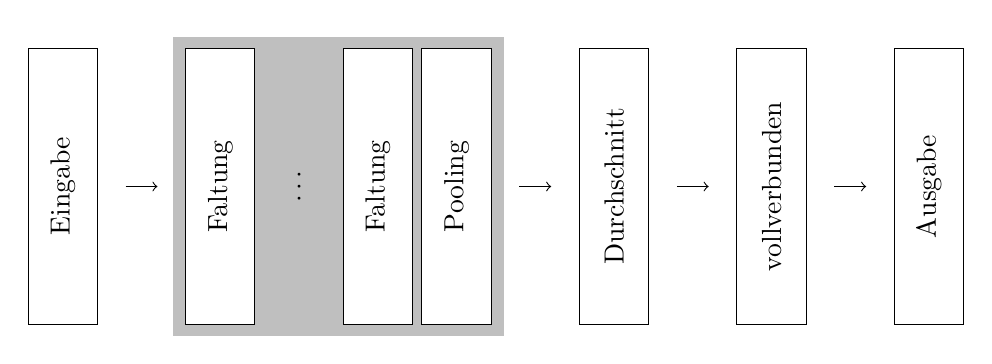
\begin{tikzpicture}[->, shorten >= 10pt, shorten <= 10pt]
  \tikzstyle{node}=[rectangle,draw, minimum width=100pt, minimum height=25pt, inner sep=0pt, fill=white, rotate=90]
  \tikzstyle{noborder}=[draw=none,fill=none]
  \tikzstyle{color1}=[fill=orange]

  \fill [lightgray] (1.4, -1.9) rectangle (5.6, 1.9) node {};

  \node[node] (0)  at (0, 0) {Eingabe};
  \node[node] (1)  at (2, 0) {Faltung};
  \node[node,noborder] (2)  at (3, 0) {$\ldots$};
  \node[node] (3)  at (4, 0) {Faltung};
  \node[node] (4)  at (5, 0) {Pooling};
  \node[node] (5)  at (7, 0) {Durchschnitt};
  \node[node] (6)  at (9, 0) {vollverbunden};
  \node[node] (7)  at (11, 0) {Ausgabe};

  \path (0) edge (1);
  \path (4) edge (5);
  \path (5) edge (6);
  \path (6) edge (7);
\end{tikzpicture}
\caption[Spektrale Netzarchitektur auf Graphen]{Typische spektrale Netzarchitektur auf Graphen bestehend aus beliebig vielen verketteten Faltungsschichten gefolgt von jeweils einer Poolingschicht.
Im Anschluss sorgt die Benutzung einer Durchschnittsschicht über den Knoten jedes Merkmals für die Verwendung von vollverbundenen Schichten hinzu zur Ausgabe.}
\label{fig:netzarchitektur_spectal}
\end{figure}

Alternative Architekturen, auch im Hinblick auf Ersetzungsmöglichkeiten des Average-Poolings, werden in Kapitel~\ref{ausblick} diskutiert.

